\chapter{Vision}
\label{cha:Vision}

\section{Motivation}
\label{sec:Motivation}
Laut einer Studie der European Environment Agency (EEA) ist Feinstaub in der Luft mitverantwortlich für den frühzeitigen Tod von ca. 66000 Menschen im Jahre 2014 \cite{AirQualityReportEEA}. Besonders in Ballungsgebieten wie Großstädten sind die gemessenen Feinstaubwerte oft am höchsten. In diesen Gebieten werden daher Maßnahmen eingeführt, die die Luftqualität verbessern sollen. Hierzu gehört z.B. die Einführung der Feinstaubplaketten im Jahr 2008 \cite{Umweltplakette}. Außerdem wurde in manchen Städten begonnen, Sensoren aufzustellen um die Umweltdaten zu messen und zu beobachten.

Ein Beispiel hierfür ist die Messstation am Heiligengeistwall in Oldenburg, die Messwerte über die Luftqualität erfasst. Am 21.10.2018 fand in der Oldenburger Innenstadt ein Marathon statt, wodurch das Gebiet um den Heiligengeistwall für Verkehr gesperrt war. Laut eines Berichts der Nordwest-Zeitung \cite{NWZMarathonOldenburg} haben Messungen der Messstation Heiligengeistwall an diesem Tag gezeigt, dass selbst ohne Verkehr der Mittelwert der gemessenen Werte nur knapp unter dem erlaubten Grenzwert lag. Der Auslöser dieser hohen Messwerte ist noch unklar. Dies kann verschiedene Ursachen haben, da beim Messen von Umweltdaten unterschiedliche Herausforderungen auftreten.

Eine dieser Herausforderungen ist zum Beispiel, dass die Messwerte stark variieren können. Umweltdaten werden immer zu einem bestimmten Zeitpunkt erfasst und spiegeln deshalb auch nur den Zustand zu diesem Zeitpunkt wieder. Es kann also vorkommen, dass ein Gebiet zur Mittagszeit eine sehr starke Umweltbelastung hat und diese zwei Stunden später schon viel geringer ist. Somit liegen in einem Gebiet nicht generell hohe Werte vor, sondern es müssen regelmäßig Umweltdaten erfasst und ausgewertet werden. Eine hohe Umweltbelastung bedeutet, dass die Messungen der Umweltdaten einen Wert annehmen, der eine negative Auswirkung auf die Gesundheit der Menschen und die Natur haben kann. Des Weiteren sind Umweltdaten von anderen Einflüssen wie z.B. Wind, Luftfeuchtigkeit und Niederschlag abhängig.

Da Menschen eine hohe Umweltbelastung, wie z.B. hohe Feinstaubwerte, nicht unbedingt wahrnehmen können, soll im Rahmen dieser Projektgruppe ein Sensorknoten konzipiert und entwickelt werden, mit dem man Informationen über die Umweltbelastungen ermittelt und der Allgemeinheit zur Verfügung stellt. Anschließend werden diese Daten ausgewertet und zur weiteren Nutzung bereitgestellt. Diese Daten können dann genutzt werden um dem Nutzer eine Möglichkeit zu bieten, Gebiete mit hoher Umweltbelastung zu umgehen und die daraus resultierenden Gesundheitsrisiken zu verringern. Deshalb werden diese ausgewerteten Daten im Rahmen des Projekts in eine Routenplanung eingespeist.

Es existiert bereits ein großes Angebot an Geräten sowie Anwendungen zur Routenplanung und Navigation. Nutzer können hiermit eine Route von einem Ort zum anderen planen und sich die schnellste oder kürzeste Strecke anzeigen lassen. Einige dieser Anwendungen lassen sogar Informationen über die aktuelle Verkehrslage in die Berechnung der schnellsten Route mit einfließen. Jedoch gibt es kaum Anwendungen, die Umweltdaten bei der Routenplanung mit einbeziehen. Würde dies geschehen, hätte es eine signifikante Verringerung der Belastung durch schädliche Umwelteinflüsse zur Folge. Bei dem obigen Beispiel der schlechten Luftqualität in Europa würde ein Routing aufgrund von Umweltdaten bedeuten, dass die Nutzer Gebiete mit gesundheitsgefährdender Luftqualität umgehen können. Außerdem werden Gebiete, die eine hohe Umweltbelastung aufweisen, sich mit der Zeit wieder normalisieren, da sie weniger befahren werden. Daraus ergäbe sich, dass die Schadstoffe nicht mehr an einem Ort konzentriert sind, sondern auf ein größeres Gebiet verteilt werden und somit das Gesundheitsrisiko gelindert wird.

Im Rahmen dieser Projektgruppe wird deshalb ein sensorbasiertes Umweltinformationssystem entwickelt, welches dem Nutzer die Möglichkeit bietet, Umweltdaten zu beobachten und eine Route zwischen zwei Orten zu planen, bei der eben diese Daten berücksichtigt werden. Zusätzlich kann entlang der geplanten Route navigiert werden.

\section{Zieldefinition}
\label{sec:Zieldefinition}
Das Ziel dieser Projektgruppe ist es, ein Produkt zu entwickeln, welches eine Navigation anhand von Umweltdaten in Oldenburg ermöglicht. Dabei besteht das Gesamtsystem global gesehen aus zwei Teilen:

Der erste Teil ist ein flexibles sensorbasiertes Umweltinformationssystem, das Umweltdaten misst, aus externen Systemen ausliest und auswertet.

Der zweite Teil ist eine Navigationsanwendung, die Umweltdaten bei der Routenplanung mit einbezieht, damit Gebiete mit starker Umweltbelastung umgangen werden.

Es muss also ein Sensornetzwerk aufgebaut werden, damit Umweltdaten gemessen werden können. Die Daten werden dann an eine IoT-Plattform gesendet und dort aufbereitet, damit Messfehler und andere Beeinflussungen bereinigt werden und qualitativ und quantitativ gute Daten für die weitere Verwendung bereitgestellt werden können. Die Navigationskomponente greift dann auf die von der IoT-Plattform bereitgestellten Daten zu und nutzt diese für die Routenplanung mit anschließender Navigation.

Hieraus ergeben sich folgende für die Umsetzung des Gesamtziels benötigten Teilziele:

\begin{enumerate}
 \item Konzeption, Entwicklung und Bereitstellung von \textbf{Sensorknoten} (siehe \Fref{sec:Sensorknoten})
 \item Entwicklung einer \textbf{IoT-Plattform} (siehe \Fref{sec:IoT-Plattform})
 \item Hohe \textbf{Datenqualität} der Umweltdaten (siehe \Fref{sec:Datenqualitaet})
 \item Entwicklung einer Komponente, die mit Berücksichtigung von Umweltdaten \textbf{Routen planen und navigieren} kann (siehe \Fref{sec:Routing_und_Navigation})
\end{enumerate}

Durch die Umsetzung der ersten drei Teilziele wird ein System erschaffen, welches Umweltdaten mit Hilfe von Sensoren misst und diese Daten nach außen zur Verfügung stellt. Es wird also der erste Teil des oben genannten Gesamtziels erfüllt. Die Erfüllung des vierten Teilziels liefert die Navigationsanwendung, wodurch der zweite Teil des obengenannten Gesamtziels erfüllt wird.

Diese Teilziele beschreiben nur die Funktionalitäten des zu entwickelnden Systems. Zusätzlich ist noch die \textbf{Erweiterbarkeit} zu betrachten. Sie beinhaltet keine weiteren Funktionen, ist aber ein wichtiges Qualitätsmerkmal, welches das System erfüllen soll. 

Die vier obengenannten Teilziele werden im Folgenden genauer beschrieben. Hierbei wird die auf Erweiterbarkeit jedes einzelnen Teilziels eingegangen.

\subsection{Sensorknoten}
\label{sec:Sensorknoten}
Das Ziel der Bereitstellung von Sensorknoten ist die flächendeckende Erfassung von Umweltdaten mit Zeit- und Raumbezug (Umweltinformationen). Exemplarisch werden mindestens 50 Sensorknoten zur Messung von Feinstaub im Oldenburger Stadtgebiet bereitgestellt. Das Gebiet ist durch einen Radius von ca. 2,5 km um den Julius-Mosen-Platz gekennzeichnet, in dem die Sensorknoten verteilt werden. Eine Bereitstellung ist grundsätzlich auch in anderen Städten und Gebieten möglich.

Um die Bereitstellung zu ermöglichen, werden Sensorknoten konzipiert und entwickelt. Diese messen verschiedene Umweltdaten und können sie an andere Systeme übertragen. Da eine hohe Anzahl an Sensorknoten bereitgestellt werden muss, sollen sie möglichst günstig sein und eine hohe Lebensdauer haben. Die Sensorknoten können zum Teil auch autark, d.h. ohne Energieversorgung durch das Stromnetz, Daten erfassen und senden, damit verschiedene örtliche Gegebenheiten berücksichtigen werden. Dazu werden sie möglichst energieeffizient konzipiert. Außerdem senden sie gemessene Werte auch nach einiger Zeit ohne Konnektivität an andere Systeme nach.

Um Messungen auch für zusätzliche Umweltfaktoren erfassen zu können, sollen die Sensorknoten darüber hinaus um weitere Sensoren erweiterbar sein.

\subsection{IoT-Plattform}
\label{sec:IoT-Plattform}
Das zweite Teilziel ist die Entwicklung einer IoT-Plattform (Internet of Things). Diese Plattform nimmt erfasste Daten aus unterschiedlichen Quellen durch beschriebene Schnittstellen entgegen und persistiert sie (Input). Außerdem bereitet sie die entgegengenommenen Daten auf und verbessert so die Datenqualität (siehe \Fref{sec:Datenqualitaet}). Darüber hinaus soll die Plattform externen Systemen und Anwendern Zugang zu den hinterlegten Daten gestatten und aggregierte Ergebnisse ermöglichen (Output).

Zusätzlich werden die bereitgestellten Sensorknoten (siehe \Fref{sec:Sensorknoten}) über die IoT-Plattform administriert. Dazu ist die eindeutige Identifikation der Sensorknoten notwendig, um diese zur Datenbereitstellung autorisieren zu können. Zudem sind Metainformationen zu jedem Sensorknoten über z.B. Betreiber, Anbringung, Betriebsdauer oder Wartungsmaßnahmen hinterlegt, um die Vertrauenswürdigkeit der gemessenen Daten besser beurteilen zu können. Die IoT-Plattform unterstützt außerdem dabei, die Wartung der Sensorknoten zu organisieren.

Außerdem soll es möglich sein neue Arten von Sensoren an der IoT-Plattform zu registrieren. Hiermit geht einher, dass die IoT-Plattform Daten über neun Umweltfaktoren entgegennehmen und persistieren kann.

\subsection{Datenqualität}
\label{sec:Datenqualitaet}
Das dritte Teilziel ist die Sicherung einer hohen Datenqualität für die repräsentable Auswertung und Darstellung von Umweltdaten. Hinsichtlich der Datenqualität wird eine hohe räumliche und zeitliche Datendichte angestrebt, um Plausibilisierungen vorzunehmen und so fehlerhafte Daten und verfälschte Auswertungen vorzubeugen. Zudem soll eine hohe Präzision (Genauigkeit und Auflösung) bei der Erfassung von Umweltdaten erzielt und systematische Messfehler bereinigt werden.

\subsection{Routing und Navigation}
\label{sec:Routing_und_Navigation}
Das vierte Teilziel ist die Entwicklung einer Navigationsanwendung, die eine optimale Route von einem Start- zum Zielort für ein gewähltes Verkehrsmittel berechnen kann (Routing). Dabei berechnet das System nicht einfach eine möglichst kurze Route, sondern berücksichtigt vor allem gesundheitliche Faktoren auf Grundlage bekannter Umweltinformationen.

Bei der Navigation wird der Nutzer entlang einer ermittelten Route geführt. Dabei erfolgt beim Abweichen von der vorgegebenen Route und durch eine veränderte Umweltsituation auf dem restlichen Weg eine Neuberechnung der Route vom Standort des Nutzers zum Zielort (dynamisches Routing). Die neue Route wird auf die aktuelle Navigation sofort angewandt (dynamische Navigation).

Im Rahmen dieses Projekts wird die Navigationsanwendung mindestens für die Stadt Oldenburg implementiert. Jedoch soll sie um andere Gebiete erweiterbar sein, wenn in diesen Gebieten die notwendigen Sensorknoten vorhanden sind.

\section{Lösungsidee}
\label{sec:Loesungsidee}
In diesem Abschnitt wird ein kurzer Überblick einer grobe Lösungsidee gegeben. Damit wird gezeigt, dass das oben genannte Vorhaben von der Projektgruppe umsetzbar ist. Hierfür wird zuerst eine grobe Architektur des zu entwickelnden sensorbasierten Umweltinformationssystems dargestellt. Anschließend wird auf die einzelnen Teilziele aus \Fref{sec:Zieldefinition} eingegangen und eine Umsetzungsidee beschrieben.

\begin{figure}[h]
	\centering
	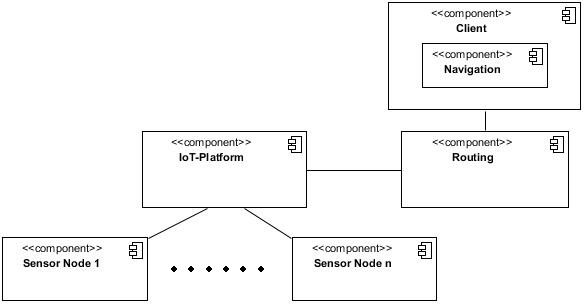
\includegraphics[width=0.75\linewidth]{ressourcen/ArchitectureFirstDraft}
	\caption{Grober Entwurf der Architektur des Systems}
	\label{fig:ArcitectureFirstDraft}
\end{figure}
In \Fig{ArcitectureFirstDraft} ist ein grober Entwurf der Architektur des zu entwickelnden Produkts zu sehen. Es besteht im wesentlichen aus vier Komponenten: dem Client, der Navigation, der IoT-Plattform und dem Sensornetzwerk.

Der \textbf{Client} ist dabei die Anwendung auf dem mobilen Endgerät des Nutzers. Hier werden dem Nutzer die verschiedenen Sensorknoten mit ihren Umweltdaten auf einer Karte angezeigt. Des Weiteren kann er gewünschten Start- und Endpunkt der Route sowie Verkehrsmittel und Umweltfaktoren angeben, die bei der Routenplanung berücksichtigt werden. Die berechnete Route wird dann auf der Karte visualisiert. Anschließend wird entlang der ermittelten Route navigiert.

Die \textbf{Routing}-Komponente reagiert dabei auf die Anfragen des Clients und berechnet die gewünschte Route für die Navigation und fordert dafür die benötigten Umweltdaten von der IoT-Plattform an.

Die \textbf{IoT-Plattform} übernimmt die Umweltdatenverwaltung. Hierfür nimmt sie die Daten von Sensorknoten und externen Systemen an, bereitet sie auf und stellt sie anschließend für die weitere Verwendung, wie z.B. die Routenplanung, zur Verfügung. Darüber hinaus werden die Sensorknoten mit Hilfe der IoT-Plattform administriert.

Ein \textbf{Sensorknoten} ist für die Messung von verschiedenen Umweltdaten verantwortlich. Mittels mehrerer Sensoren für verschiedenartige Umweltfaktoren erhebt er Messwerte, die er an die IoT-Plattform sendet.

Im Folgenden werden die Lösungsideen für die Teilziele aus \Fref{sec:Zieldefinition} erläutert.

\subsection{Sensorknoten}
\label{sec:SensorknotenLoesung}
Ein Sensorknoten ist eine Komposition, die aus einem Verarbeitungssystem und mehreren Messsystemen besteht. Dabei besteht das Verarbeitungssystem aus einer Steuer- und Kommunikationseinheit. Die Messsysteme sind Sensoren, die die Umweltdaten messen. Im Rahmen der Projektgruppe werden vorhandene Sensorknoten untersucht. Insbesondere der Feinstaubsensor des Projekts \textit{luftdaten.info} des \textit{OK Lab Stuttgart} \cite{luftdateninfo} soll weiterentwickelt werden, aber gleichzeitig kostengünstig bleiben. Der Energieverbrauch des Sensorknotens soll verringert werden, damit er möglichst lange mit einer stationären Energieversorgung (z.B. Powerbank) betrieben werden kann. Zusätzlich soll eine Pufferung der Messwerte stattfinden, um auch bei zeitweisem Konnektivitätsverlust die gemessenen Werte nachzusenden.

Diese verbesserten Sensorknoten werden in möglichst großer Anzahl im Oldenburger Stadtgebiet angebracht und an der IoT-Plattform registriert, damit Umweltdaten für die Routenplanung in Oldenburg bereitstehen.

\subsection{IoT-Plattform}
\label{sec:IoT-PlattformLoesung}
Es wird eine Plattform geschaffen, die Schnittstellen für Sensorknoten und externe Systeme bereitstellt. Darüber lassen sich Messwerte an das System übertragen, welche persistiert und den Sensorknoten zugeordnet werden. Die IoT-Plattform kann diese Daten dann aggregieren und über weitere Schnittstellen im Anschluss für andere Dienste bereitstellen.

Zusätzlich gibt es eine Administrationsoberfläche, über die Identifikation, Autorisierung sowie Pflege von Metainformationen der einzelnen Sensorknoten ermöglicht wird. Darüber hinaus können Benachrichtigungen konfiguriert werden, wie z.B. Mailversand bei fehlendem Dateneingang, um die Wartung der Sensorknoten besser zu organisieren.

\subsection{Datenqualität}
\label{sec:DatenqualitaetLoesung}
Die verwendeten Daten zur Routenberechnung sollen von hoher Qualität sein. Um eine hohe zeitliche Dichte zu gewährleisten, senden die Sensorknoten ihre Messwerte in möglichst kurzen Intervallen. Für die räumliche Dichte werden die Sensorknoten sinnvoll im Oldenburger Stadtgebiet verteilt. Darüber hinaus verwendet das System virtuelle Sensorknoten, die für einen bestimmten Standort die Messwerte der umliegenden Sensoren einspeisen und zusätzlich weitere Einflussfaktoren der örtlichen Gegebenheiten berücksichtigen.

Damit fehlerhafte Daten und verfälschte Auswertungen vermieden werden, sind statistische Verfahren zur Datenbereinigung anzuwenden (z.B. das Streichen von Ausreißern).

Systematische Messfehler werden durch die Verwendung von Sensorfusion bereinigt, indem verschiedene Umweltdaten zur Korrektur eines anderen Messwertes herangezogen werden. Dies ist erforderlich, da Messergebnisse von einigen Einflussfaktoren abhängig sind, die ihre Genauigkeit beeinflussen. So ist z.B. bekannt, dass die Feinstaubsensoren von \textit{luftdaten.info} bei hoher Luftfeuchtigkeit zu hohe Werte liefern \cite{luftdateninfoMessgenauigkeit}. Durch die Bestimmung und Analyse dieser Einflussfaktoren wird erhofft, dass der falsch ermittelte Feinstaubwert unter Berücksichtigung der Luftfeuchtigkeit korrigiert werden kann.

\subsection{Routing und Navigation}
\label{sec:Routing_und_Navigation_Loesung}
Die Route soll anhand der gemessenen Umweltdaten berechnet werden und folglich eine geringe Umweltbelastung aufweisen. Dazu kann der Nutzer vor der Ermittlung einer Route seine gewünschten Umweltfaktoren angeben, die in die Berechnung einfließen sollen. Liegen auf einem Teilweg schlechte Werte zu den gewählten Umweltfaktoren vor, so wird dieser Teilweg mit einem Strafgewicht versehen. Die berechnete Route enthält dann möglichst geringe Strafen und ist gleichzeitig kurz bzw. schnell. Die Visualisierung wird in einem existierenden Kartentool, zum Beispiel Google Maps oder OpenStreetMap, vorgenommen.

Bei der Navigation werden Standortdaten des Nutzers verwendet, damit auf Abweichungen von der vorgeschlagenen Route mit einer Neuberechnung reagiert werden kann. Zudem werden die Umweltdaten auf der vorliegenden Restroute regelmäßig auf starke Veränderungen überprüft, um den Nutzer bei plötzlicher hoher Belastung darüber zu informieren.
%
%\newpage
%\section{Glossar}
%\label{Glossar}
%
%\textbf{Navigation:}
%Navigation ist die Leitung eines Nutzers entlang einer berechneten Route.\\
%\\
%\textbf{Routing:}
%Routing ist ein Verfahren, in welchem aufgrund von Umweltdaten eine Strecke von einem eingegebenen Start- und Endpunkt berechnet wird.\\
%\\
%\textbf{Dynamisches Routing:}
%Dynamisches Routing ist ein Verfahren, in welchem aufgrund von veränderten Umweltdaten die Route während der Navigation neu berechnet wird.\\
%\\
%\textbf{Dynamische Navigation:}
%Dynamische Navigation ist die Anpassung der Leitung des Nutzers entlang der Route. Diese Anpassung erfolgt aufgrund der Nichteinhaltung der Route oder aufgrund der Auswahl einer alternativen Route, die aufgrund des dynamischen Routings zur Verfügung steht.\\
%\\
%\textbf{IoT:}
%IoT ist die Abkürzung für \dq Internet of Things\dq  und ist ein Sammelbegriff für Technologien einer globalen Infrastruktur der Informationsgesellschaften, die es ermöglicht, physische und virtuelle Gegenstände miteinander zu vernetzen und sie durch Informations-und Kommunikationstechniken zusammenarbeiten zu lassen.\\
%\\
%\textbf{Sensor:} Ein Sensor ist ein technisches Bauteil, das bestimmte physikalische (oder chemische Eigenschaften) seiner Umgebung qualitativ oder als Messgröße quantitativ erfassen kann.\\
%\\
%\textbf{Sensorknoten:} Ein Sensorknoten ist eine Komposition bestehend aus einem Verarbeitungssystem und mehreren Messsystemen. Dabei besteht das Verarbeitungssystem aus einem Controller und einer zugehörigen Kommunikationseinheit. Das Messsystem sind Sensoren, die die Umweltdaten messen, wie zum Beispiel Luftdruck, Feinstaub oder Temperatur. \\
%\\
